\documentclass[twoside,single]{lion-msc}

\title{Summer Research Internship 2017}
\author{Mudit Garg}

\affiliation{Indian Institute of Technology Delhi}   % this is the default value
%\affiliation{Instituut-Lorentz, Leiden University}                     % for theoretical physics
\usepackage{float}
%\affiliation{Huygens-Kamerlingh Onnes Laboratorium, Universiteit Leiden}   % experimental physics in Dutch
%\affiliation{Instituut-Lorentz, Universiteit Leiden}                       % theoretical physics in Dutch
\id{Senior Undergraduate}
\address{New Delhi, India, 110016}               % default address - uncomment if need be
\usepackage{amssymb} 
\usepackage[export]{adjustbox}
% \newdate{date}{\day}{\month}{\year}           % definition of time and date using datetime package
%\newdate{date}{27}{08}{2010}
%\date{\displaydate{date}}
\usepackage{enumerate}
\studentid{May-July 2017}                           % check you student ID, LaTeX does not do this
\abstract{I would like to express my deep gratitude toward \textbf{Prof. Michel Orrit} for giving me this wonderful opportunity to spend my Summer at Single Molecule Group and for his constant guidance.I would like to thank \textbf{Biswajit Pradhan} for his daily supervision and constructive discussions .\\~\\
This research internship was made possible by financial support from the \textbf{Leiden University} and I am thankful for that.I am certainly grateful to \textbf{Prof. Jan Aarts} for coordinating my summer internship and taking care of all logistics.
\\~\\Special thanks to \textbf{MoNOS} group for accepting me in their family and helping me into smooth transition in leiden.I've gained so much experience and knowledge here that can't be expressed in words. \\~\\
Also I  would like to express my gratitude toward  \textbf{Prof. R.K. Soni}, the internal supervisor of this internship with his ever-helping nature and support.   }     % limit your self to 1/2 page or 500 words
\supervisor{Prof. Dr. Michel Orrit}                         % Note that this should be a LION staff member!
\dsupervisor{Biswajit Pradhan}                      % This could be a LION staff member or your external supervisor

\degree{Research Internship}                     % The default option is "Bachelor of Science", change if needed


\major{Single-Molecule Optics Group,LION}                  % The default option is "Physics", change if needed
%\major{Physics and Mathematics}

% optional cover picture - should be jpg or pdf

\coverpicture{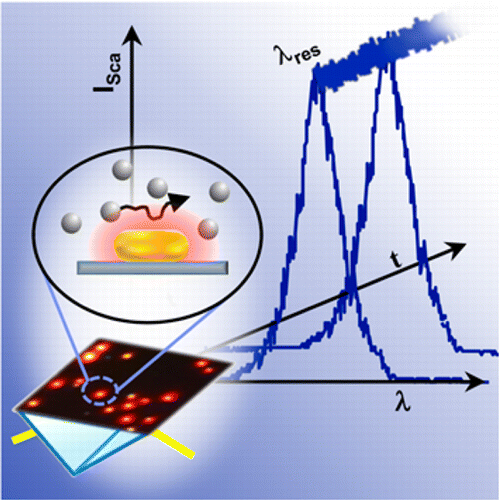
\includegraphics[width=8cm]{1.png}} 


% Use this to make hyperlinks visible in the document.
% \hypersetup{colorlinks=true}

% ---------------------------------------------------------------- My defintions!
% \renewcommand{\vec}[1] {\ensuremath{ \overrightarrow{ #1 } }}
\renewcommand{\vec}[1] {\ensuremath{ \mathbf{ #1 } }}
% \bra \ket \braket and \proj
\newcommand{\bra}[1]{\ensuremath{\langle #1 \vert}}
\newcommand{\ket}[1]{\ensuremath{\vert #1 \rangle}}
\newcommand{\braket}[2]{\ensuremath{\langle #1 \vert #2 \rangle}}
\newcommand{\proj}[1]{\ensuremath{\vert #1 \rangle \langle #1 \vert}}

\newcommand{\kpar}{\ensuremath{k_\parallel}}
% ----------------------------------------------------------------

% \usepackage{tocloft}
% \renewcommand{\cftchapdotsep}{\cftdotsep}

\begin{document}

% roman numbering in the table of contents section
\pagenumbering{roman}


\maketitle

% Table of contents :  it is a good idea to include this into your thesis
\tableofcontents
\cleardoublepage

% The following list of figures and list of tables are optional. Remove the comments if needed
%\listoffigures
%\newpage

%\listoftables
%\newpage

% in the main part of the document use standard arabic numbers. Page counter resets to 1.
\pagenumbering{arabic}

\chapter{Introduction}

The determination of size of small biomolecules like protein is important in biochemical and pharmaceutical studies. Dynamic light scattering(DLS) is usually used to  measure the sizes of colloidal nanoparticles. But the determination of sizes of small biomolecules by DLS is not very reliable. Surface plasmon resonance(SPR) of nanophotonics structures like gold nanorod(AuNR), bipyramid is sensitive to the refractive index of its local environment. Single protein can be detected using the shift in SPR of nanostructures\cite{AuNR4}. Here in this project we used scattering intensity of AuNR to detect freely diffusing protein. We intend to measure size and concentration of protein from the correlation of scattered intensity of AuNR.
\chapter{Theory}

\section{Fluorescence}
Fluorescence is the property of substance where it absorbs light at certain  wavelength and emit light at relatively longer wavelength,Therefore have lower energy than the absorbed one. The molecule is termed as fluorophore or fluorescent dye. It happens in three stages : First excitation then vibrational relaxation and finally fluorescence emission. This is displayed using Jablonski diagram.

\begin{figure}[H]
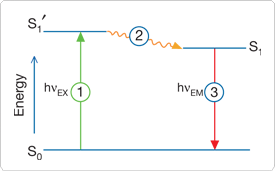
\includegraphics[width=.5\textwidth,center]{2}
\caption  {Jablonski diagram illustrating the three stages of fluorescence.In the first stage photon of energy $h\nu_{EX}$ is supplied by laser and absorbed by  fluorophore, which results in excited electronic singlet state ${S_1}'$.Then it stays in that state for finite duration(1-10 ns).In second stage, flurophores undergoes conformational changes which results in partial dissipation which yields relaxed singlet excited stage $S_1$. In final stage a photon of energy $h\nu_{EM}$ emits returning the flurophores back to $S_0$. \cite{AuNR2}}
\end{figure}

The emitted photon has less energy then the absorbed one. The difference $h\nu_{EX}-h\nu_{EM}$ is called stokes shift. Stokes shift allows the emission photons to be detected against a low background, which can be easily separated from excitation laser.

\section{Fluorescence Correlation Spectroscopy}
Fluorescence Correlation Spectroscopy(FCS) is a technique which can be used to monitor single molecule using a confocal microscope. In this setup we send laser beam to this microscope's objective via Beam splitter,which is focus to its diffraction limited volume on the sample. Then we collect the fluorescence light form this and send it to pin hole. This goes through emissions filters and beam splitter and finally to detectors. Few nanomolars of fluorescence are used in order to detection of single molecule.  The formula for normalized autocorrelation of intensity traces I(t) is :
$$
G(\tau) = \frac{\langle{I(t)}\cdot{I(t+\tau)}\rangle}{\langle{I(t)}\rangle^2} 
$$
and if we define $\delta{I(t)} = I(t) - \langle{I(t)}\rangle$ then $G(\tau)$ can be written as :
$$	
G(\tau) = \frac{\langle\delta{I(t)}\cdot\delta{I(t+\tau)}\rangle}{\langle{I(t)}\rangle^2} +1
$$
It is given in more details in reference \cite{AuNR3}

\newpage
\section{Scattering Correlation Spectroscopy(SCS}
In SCS technique\cite{AuNR1}, we monitor the scattered intensity from immobilized single AuNR. We use flow cell to control the environment of the AuNR. Then we introduce diffusers such as small gold.We measure the intensity of the AuNR as diffusers enter and leaves in its vicinity. Then we take autocorrelation of intensity I(t) to find out diffusion coefficient D. Then using stokes einstein relation $ D = \frac{k_B{T}}{6\pi\eta{r}}$ we can find viscosity and diffuser conc. of other diffusers if we know it for one using their respective D.

\begin{figure}[H]
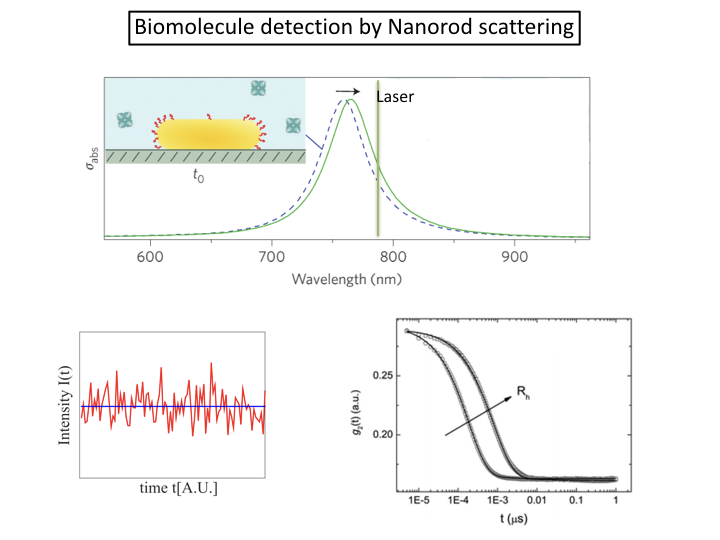
\includegraphics[width=1\textwidth,left]{13}
\caption {Protein is diffusing freely in the solution,Dotted line shows the spectrum of AuNR and solid line shows a shift in SPR whenever protein comes near the tip of AuNR.There are bursts in the time trace whose autocorrelation shows clear decay. The correlation decay time should change as a function of the size( $R_h$) of the molecule \cite{AuNR4}}
\end{figure}

\begin{figure}[H]
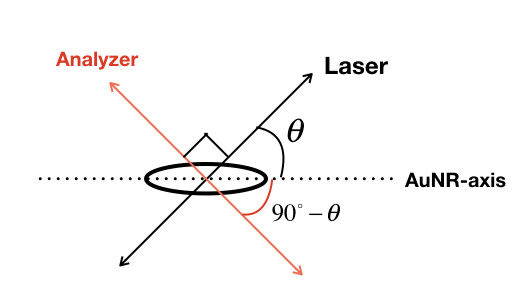
\includegraphics[width=1\textwidth,left]{9}
\caption {Laser is at an angle $\theta$ with axis of AuNR and perpendicular to analyzer which is extinguishing the reflection part (
$ I_{reflection} = I_{L}\cdot\cos90^{\circ} = 0$) .so only scattering along the axis survive and result in final intensity.}
\end{figure}
$$
I_{total} = Reflection+AuNRscat = 0 +   I_{scatAuNR}\cdot\cos(90^{\circ}-\theta)
$$
$$
I_{total} = I_{scatAuNR}\cdot\sin(\theta)
$$
The angle $\theta$ can be varied to get better signal fluctuation \& hence correlation

\chapter{Experiment}
This is my full procedure in the internship:

\section{Sample Preparation}
 \begin{enumerate}[I]
   \item I first prepared sample using stock AuNR solution which were coated with CTAB to avoid aggregates
   \item I only chose those solution which have surface plasmon resonance around 650 so that they right wing at 660 nm.
   \item then remove CTAB using centrifugation.This is necessary so that AuNR could stuck glass slides.
   \item then I sonicated the sample to avoid aggregates.
   \end{enumerate}
  \section{Putting AuNRs on glass slide}
   \begin{enumerate}[I]
   \item After that I used two different way to prepare AuNR sample
   \begin{enumerate}[i]
   \item Flow cell with rectangular slide
   \item Circular holder with circular slides
   \end{enumerate}
   \item Also used two different procedure for introducing AuNR to glass slides
   \begin{enumerate}[i]
   \item Spin coating method 
   \item Immobilization on thilated surface
   \end{enumerate}
   \end{enumerate}
  \section{Microscopy}
     \begin{enumerate}[I]
   \item  So I used this setup for experimenting
   \begin{figure}[H]
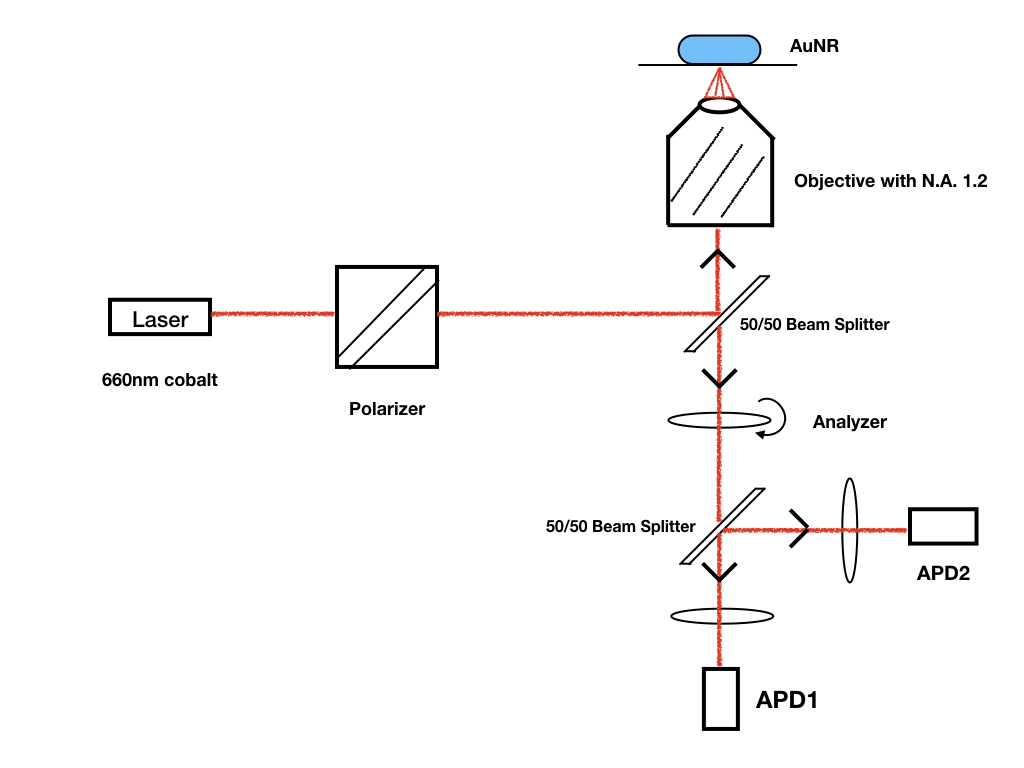
\includegraphics[width=1.1\textwidth,left]{10}
\begin{flushleft}
\caption{In this Experimental setup laser is going through polarizer then using 50/50 beam splitter going to AuNR though microscope and coming back through analyzer which is then again splitting by 50/50 beam splitter to APDs. }
\end{flushleft}
\end{figure}
   \item I took scattering image using 660 nm red laser at focus for finding out positions of AuNR.
   \item Then I took spectrum using 532nm green laser for those AuNR which were visible by 660 nm.
   \item After doing this process I chose those AuNRs which had SPR either right wing or left wing at 660 nm.
   \item then I passivated the AuNRs with either Thioglycolic acid or Cysteamine to avoid nonspecific sticking between protein and AuNR.
   \item Then after leaving it for overnight I introduced different concentrations of BSA protein.
   \item Took their time traces using signal form the two APDs.
   \end{enumerate}
   \section{Analysis}
   \begin{enumerate}[I]
   \item I calculated their cross correlations using intensity traces in order to find diffusion time.
   \item and finally using Stokes Einstein relation to find out size of protein.
    \end{enumerate}
  
\chapter{Results and Discussion}

So I would like to share my two days of result in which laser was stable.So in first case I passivated with 20$\mu$M Cysteamine and in second case with 100 $\mu$M Thioglycolic acid.

\section{Passivation with 20$\mu$M Cysteamine}
\begin{figure}[H]
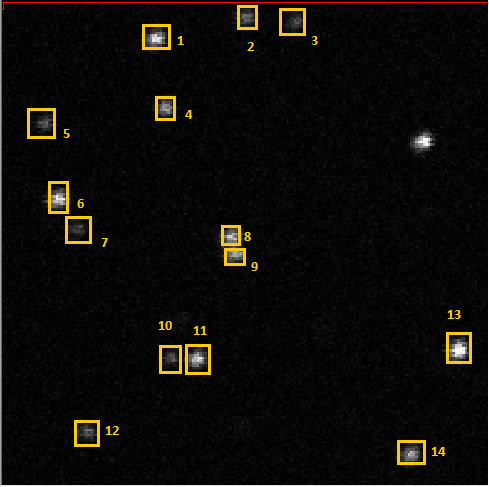
\includegraphics[width=.6\textwidth,center]{3.png}\\
\caption {660 nm scattering image of 20$\mu$m$\times$20$\mu$m area passivated with Cysteamine.Numbering according to order of taking spectrum}
\end{figure}
Out of these fifteen only ten i.e. 2,3,5,6,8,10,12,13,14,15 had right spectrum.
then I introduced 100nM BSA.Then took 300 second time traces.After doing that I again took the spectra and found out that there was a shift of 2-3nm in SPR and decrease of around 1nm in FWHM.
\begin{table}[H]
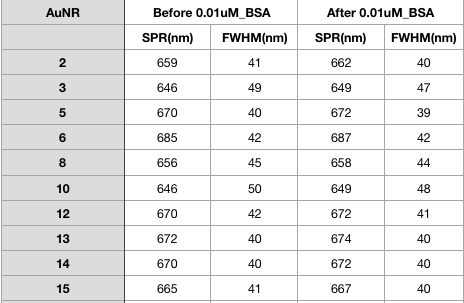
\includegraphics[width=1\textwidth,center]{4.png}\\
\caption {There is a redshift in SPR of every AuNR after adding BSA and also a decrease in FWHM.This shows that BSA is sticking to the AuNR}
\end{table}
\newpage
I would particularly discuss one of the AuNR which was showing some correlation i.e. AuNR6
\begin{figure}[H]
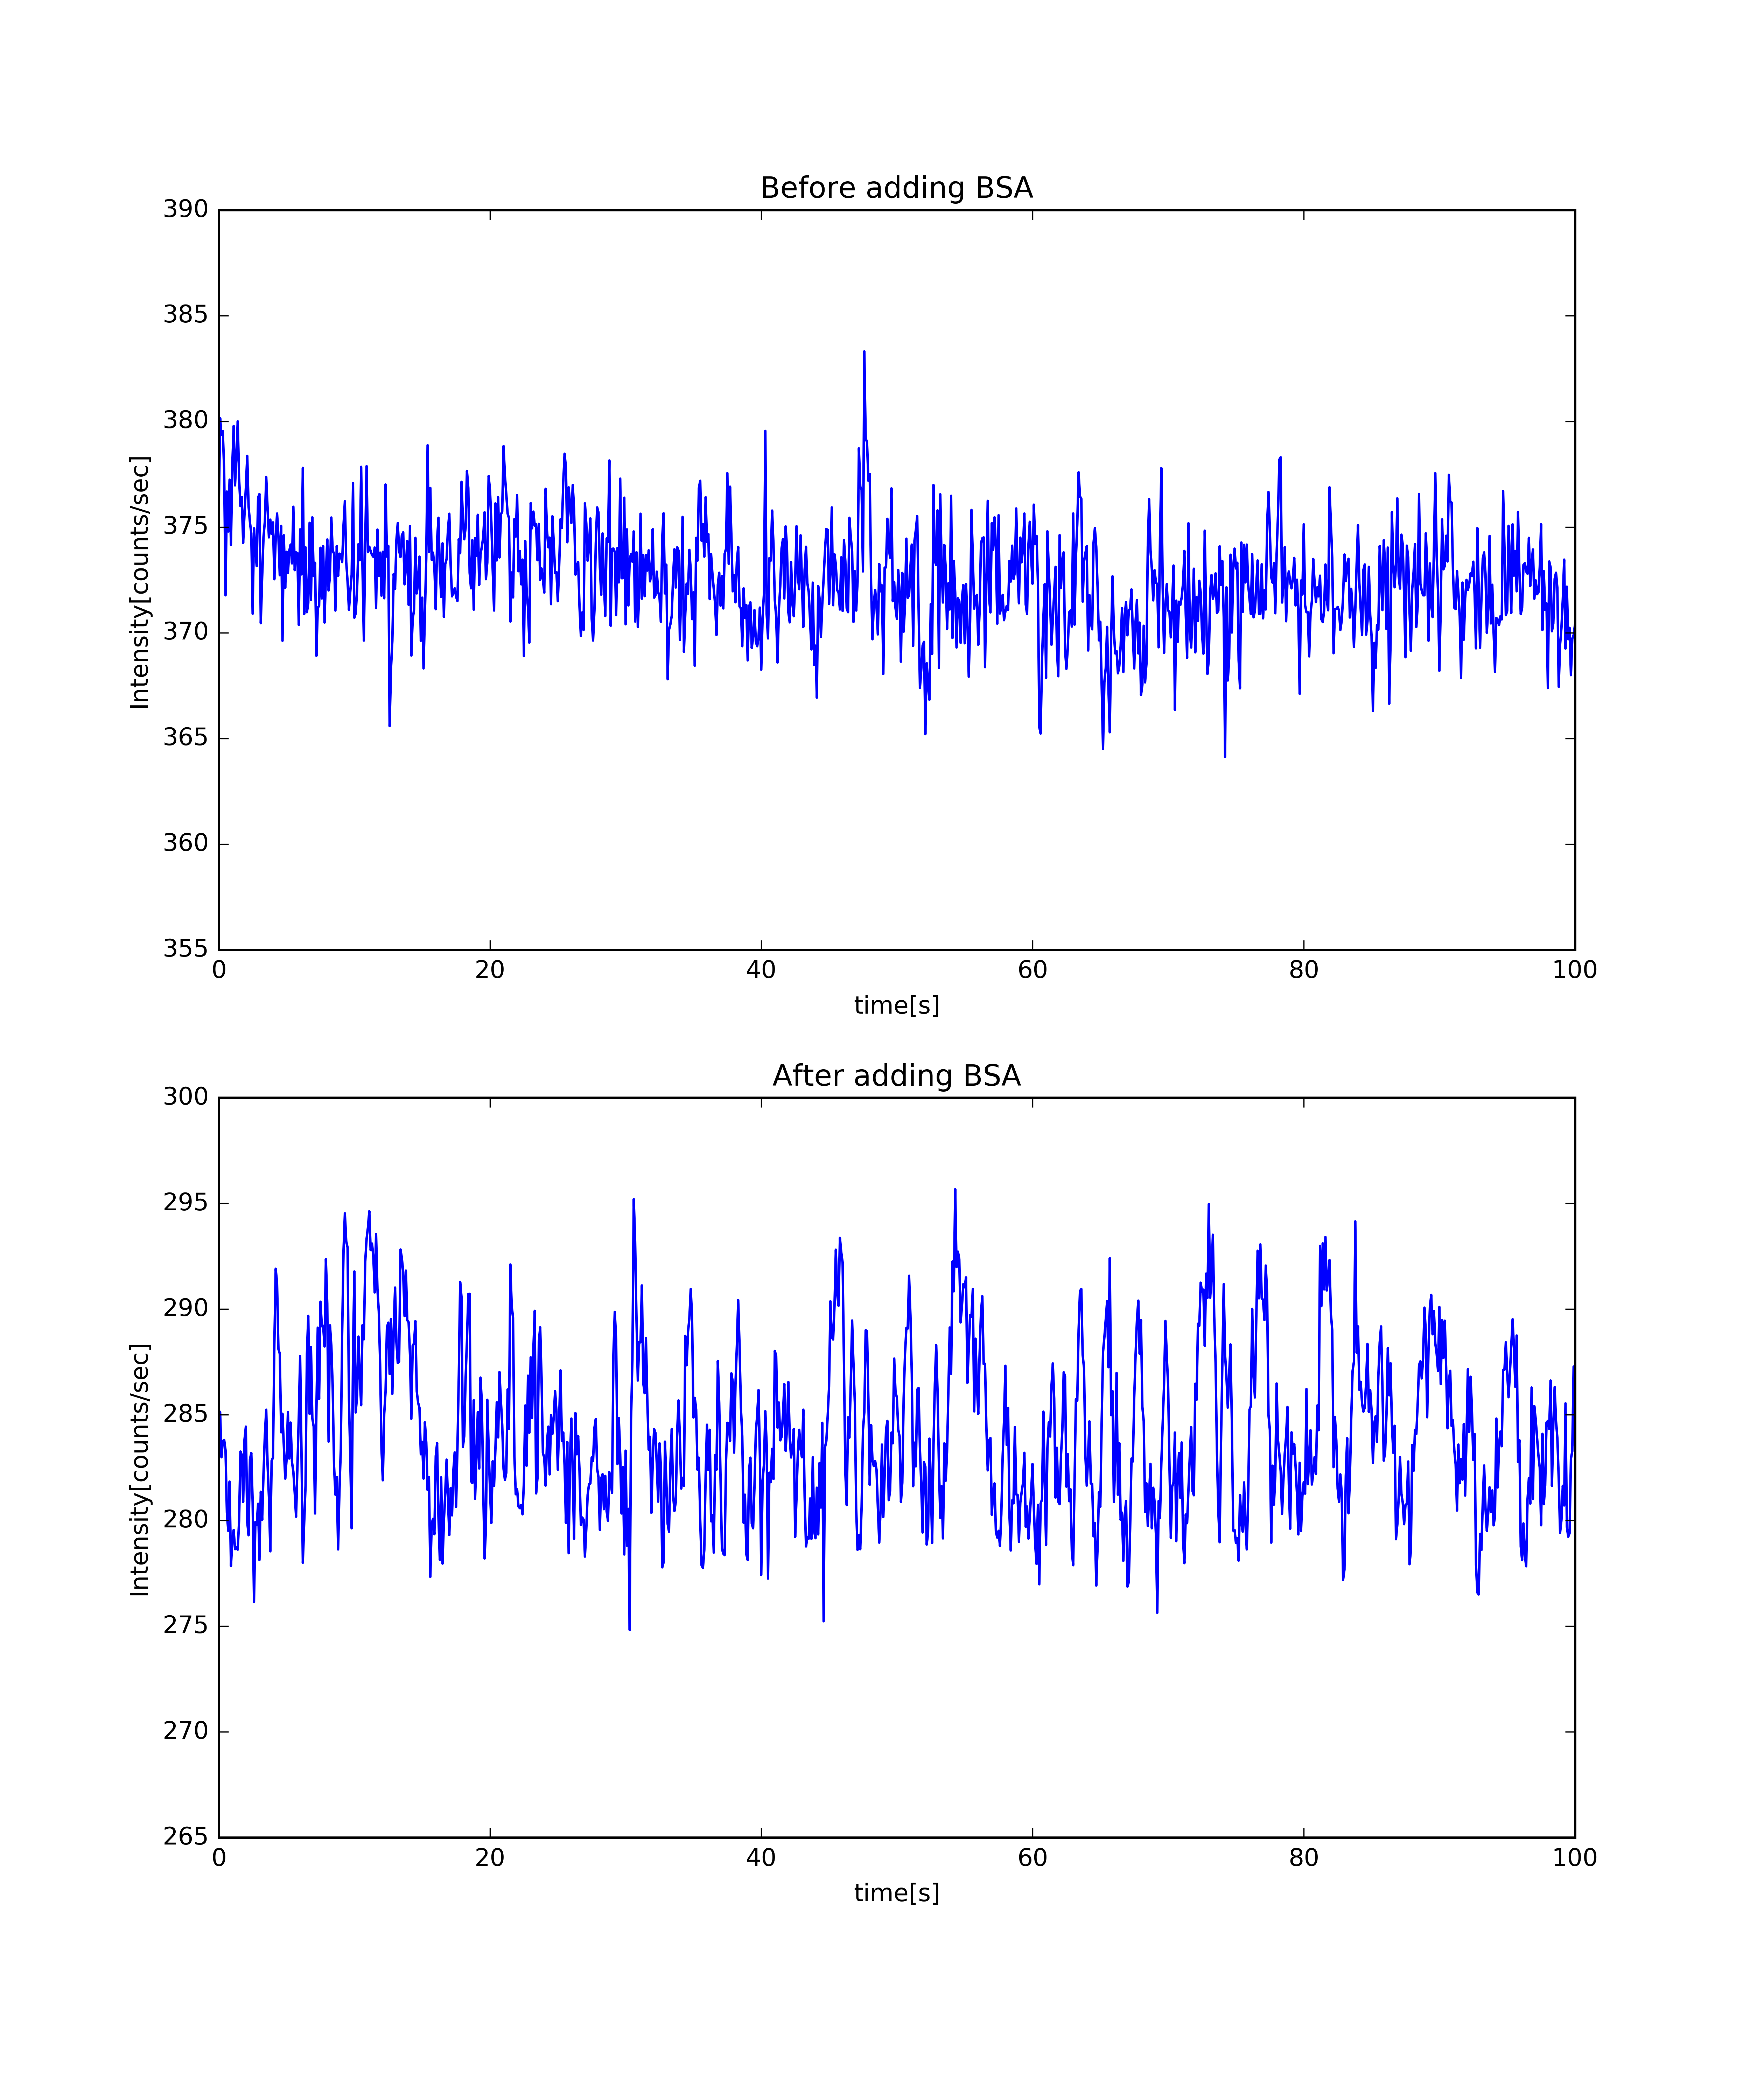
\includegraphics[width=1\textwidth,center]{11}
\begin{center}
\caption {Time Trace of AuNR6 before and after BSA.As we can see from time traces that due to BSA there are more fluctuations in same period which shows that scattering intensity is sensitive to protein sticking}
\end{center}
\end{figure}
\begin{figure}[H]
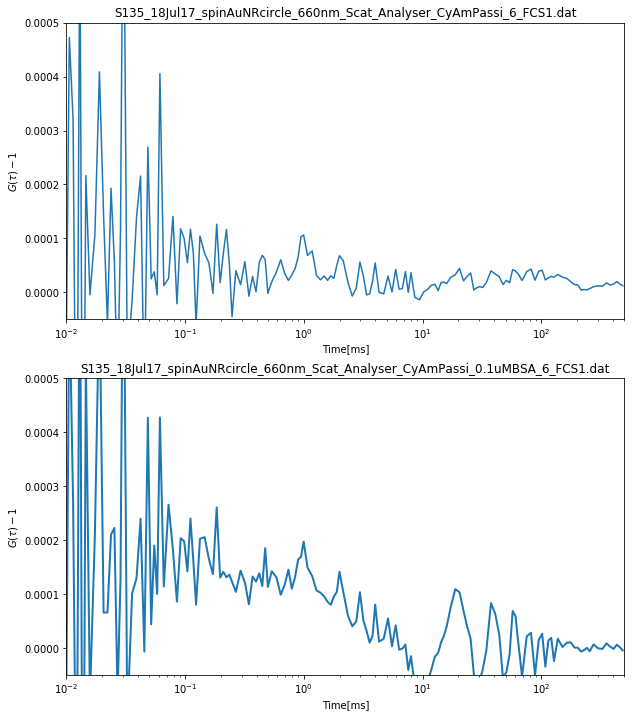
\includegraphics[width=.6\textwidth,center]{12}
\begin{center}
\caption {FCS correlations of AuNR6 before and after BSA.There is some correlation due to the some sticking of BSA. The correlation time is 1.8ms which is very different from the expected value of 10 s of $\mu$sec. This longer time can be attributed to the sticking of the protein.}
\end{center}
\end{figure}

\begin{figure}[H]
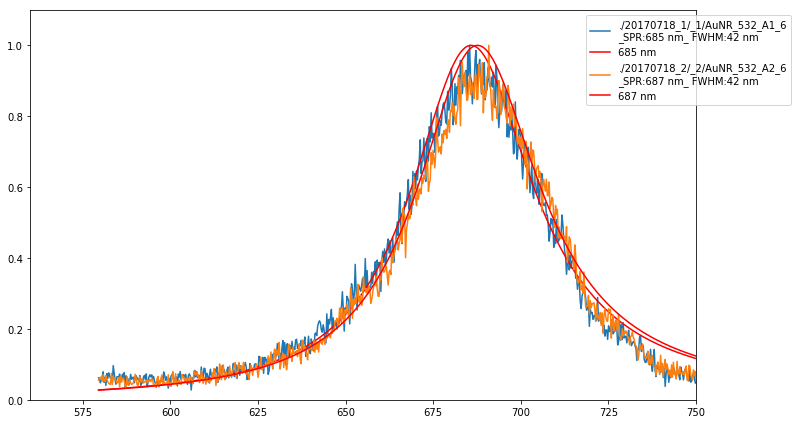
\includegraphics[width=.6\textwidth,center]{7}
\begin{center}
\caption {Spectrum shift in AuNR6 before and after adding BSA to AuNR environment.There is redshift of 2nm in SPR which tells us that there is sticking of BSA to AuNR.}
\end{center}
\end{figure}
\section{Passivation with 100$\mu$M Thioglycolic acid}
\begin{figure}[H]
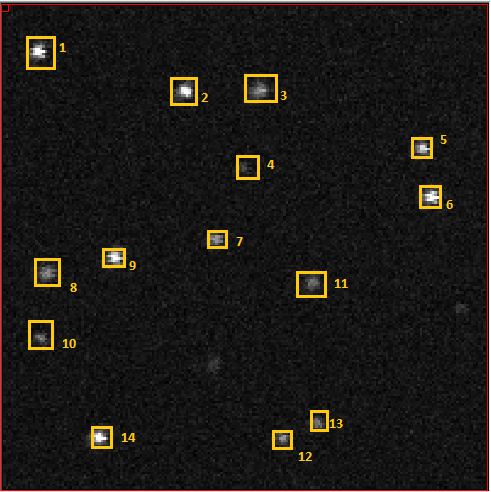
\includegraphics[width=.6\textwidth,center]{6.png}\\
\caption {660 nm scattering image of 20$\mu$m$\times$20$\mu$m area passivated with Thioglycolic acid.Numbering according to order of taking spectrum}
\end{figure}
Out of these fourteen only nine i.e. 1,3,4,6,7,10,11,12,13 had right spectrum.
then I introduced 1nM BSA.Then took 600 second time traces.After doing that I again took the spectra and found out that there was a shift of 2-3nm in SPR and but his time increase of around 1nm in FWHM.
\begin{table}[H]
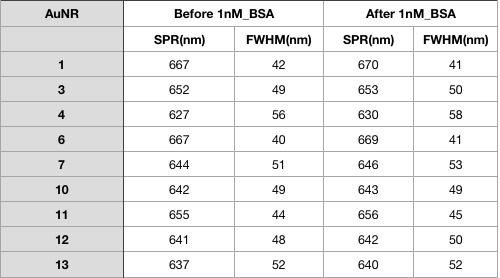
\includegraphics[scale=.6]{5.png}\\
\caption {There is a redshift in SPR of every AuNR after adding BSA and also a decrease in FWHM.This shows that BSA sticking to AuNR}
\end{table}

As I laid out in my in previous discussion,I was not able to achieve proper correlation due to the following reasons.
\begin{enumerate}
\item Initially laser wasn't stable which gave is erroneous results.
\item Not able to prevent sticking of BSA to AuNR
\item Time constraint of my internship
\end{enumerate}
Due to this time constraint I spent my initial time learning the technique and how to make samples.After that we found out that our 670 nm laser is not stable,so we ordered a new one 660nm cobalt laser but even after accelerating the procedure it took 3 weeks to arrive.even after finally setting up the laser which was stable.we weren't able to avoid attaching of BSA even after the passivation.

\section{Conclusion}
First conclusion is that we're experimentally able to detect protein sticking by scattering measurement. Second conclusion is that due to only a change of 3-4 \% intensity in time trace after introduction of BSA ,FCS correlation is too noisy which hinders our ability to analyze.
 
\section{Outlook}
We can use good detectors which have low photon noises such as photodiode to get better correlations. Also we can passivate AuNR better to avoid sticking with protein. The polarization angle of excitation laser can be optimized to achieve maximum sensitivity.
\bibliographystyle{lion-msc}
\bibliography{Thesis}

\end{document}

